\section{Implications}


% - Explain biases based on these models
\begin{frame}[c]{Implications - Models}
    \Large
    Your brain is creating predictive models for everything. \\ \\
    \pause
    You are only familiar with what you have already thought about. \\ \\
    \pause
    Learning is the active creation of new models (spatial and temporal patterns).
\end{frame}


% - requiring ten times more resources during learning
\begin{frame}[c]{Implications - Learning}
    \Large
    While Learning, you need about 90 percent more capacity than after having mastered something. \\ \\
    \pause
    % - AHA-Moment (aligning models, ceasing bursting)
    'AHA-Moment' is when models line up, and bursting ceases. \\ \\
    \pause
    % - Explain the fact that smarter people have less Brain activity
    Smarter people have clearer models and have less overall brain activity (higher efficiacy).
\end{frame}


% - explain gradient for Einstein/Craziness, proving vs disproving in the brain -> THC is bad
\begin{frame}[c]{Implications - Brain Parameters}
    \Large
    There is also a varying threshold for the spatial pooler activations. \\ \\
    \pause
    This probably also changes during sleep.
\end{frame}


% - explain 'top-down' phenomena and common biases

\begin{frame}[c]{Implications - Conformation Bias}
    \Large
    Conformation Bias is a predictable result from the temporal pooler.
\end{frame}


% - Mistakes that happen by top-down enforcing (e.g. the dalmatine picture, scrambled words)
\begin{frame}[c]{Implications - Inhibition in the Visual System}
    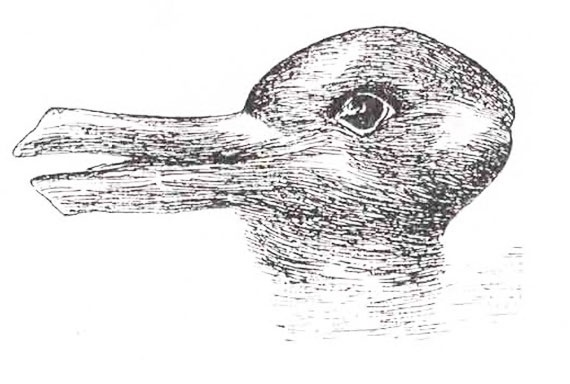
\includegraphics[width=\textwidth]{rabbit_duck}
\end{frame}


% - Context-dependent processing
\begin{frame}[c]{Implications - Inhibition in the Visual System}
    
\includegraphics[height=\textheight]{The_Dress}
\end{frame}



\begin{frame}[c]{Implications - Top-Down Processing I}
    \Large
    Yuo cna porbalby raed tihs esaliy desptie teh msispeillgns. \\ \\
    \pause
    A vheclie epxledod at a plocie cehckipont near the UN haduqertares in Bagahdd on Mnoday kilinlg the bmober and an Irqai polcie offceir
\end{frame}


\begin{frame}[c]{Implications - Top-Down Processing II}
    \Large
    Aoccdrnig to a rscheearch at Cmabrigde Uinervtisy, it deosn’t mttaer in waht oredr the ltteers in a wrod are, the olny iprmoetnt tihng is taht the frist and lsat ltteer be at the rghit pclae. The rset can be a toatl mses and you can sitll raed it wouthit porbelm. Tihs is bcuseae the huamn mnid deos not raed ervey lteter by istlef, but the wrod as a wlohe.
\end{frame}


% - explain gradient for Autism and that it is more 'bottom up'
\begin{frame}[c]{Implications - Bottom-Up-Gradient}
    \Large
    There is a parameter for how much predictive states count for the spatial pooler. \\ \\
    \pause
    Which one would be better? \\ \\
    \pause
    Possibility: Predictive states count less for Autistic people.
\end{frame}


% - explain theory: inhibited-boost: hallucination
\begin{frame}[c]{Implications - Hallucinating}
    \Large
    Hallucinating is just active boosting in the human brain. \\ \\
    \pause
    Concentration going awry as well ... \\ \\
    \pause
% - Phantom limb 'pain' -> boosting
    Phantom limbs ...
\end{frame}


\begin{frame}[c]{Implications - Reticular Activating System}
    \Large
    Ever noticed after buying something, \\
    everyone has the same thing?
\end{frame}


% - Explain Priming based on predictive stuff (the priming-bias)
\begin{frame}[c]{Implications - Priming Bias}
    \Large
    \pause
    Priming really leaves some predictive states, even though it never gets
    high enough in the hierarchy to notice it consciously.
\end{frame}


% % - Explain the bayesian-reasioning part
% \begin{frame}[c]{Implications - Bayesian Reasoning}
%     \Large
%     The brain is constantly weighing alternatives and selecting the likeliest - as far as it is aware.
% \end{frame}


\begin{frame}[c]{Implications - Cached Thought}
    This fully explains the fallacy of cached thought, among others.
\end{frame}


% - Implications on Meaning (?)
\begin{frame}[c]{Implications - Meaning}
    \Large
    Something has meaning if it is a well-connected concept.
\end{frame}





% - Mistakes that happen by accidential correlation: search for good example; mistaking something to be true



% - Introduce HTMv3 !
% - Motor movements are just very strong predictions the body 'makes happen'
%   - Flow state is where everything is exactly as predicted
% - Location-based composition: This explains mind palaces!
% - Everything is a 'conceptspace' -
% - Explain how cortical columns create quite powerful models


